\section{Plano de Trabalho e Cronograma de Excecução}

Assim, são determinadas as seguintes tarefas para essa proposta:

\begin{itemize}
    \item[\textbf{T1 }] Estudo aprofundado sobre MEC e MCGI monocomponentes pré-existentes na literatura.% Sobre o MEC, estão incluidos o estudo da derivação dos modelos de Abramzon-Sirignano \cite{Sirignano1989}, a formulação de Miller \cite{MillerR1998}, \todo{...}, No que tange a MCGIs, revisitar o modelo de Godsave-Spalding \cite{Law1978,HenningsJ2024MT}, estudar o artigo do Fachini \cite{FachiniF1999}, suas referências e citações, \todo{...} 
    \item[\textbf{T2 }] Modelagem analítica de combustão de gota isolada monocomponente com modelo avançado de evaporação.% Essa tarefa baseia-se na incorporação do modelo de Abramzon-Sirignano \cite{Sirignano1989} ou da formulação de Miller \cite{MillerR1998} no modelo de Godsave-Spalding \cite{Law1978}. %Como todos os modelos citados baseiam-se em soluções analíticas, é visto como provável que 
    \item[\textbf{T3 }] Estudo de modelos pre-existentes para a modelagem  analítica de discretização do interior de gota monocomponente.% São exemplos de literatura relevante para essa tarefa \source{}.
    \item[\textbf{T4 }] Avaliação da viabilidade de acoplamento de modelos monocomponente de combustão de gota isolada com discretização no interior da gota.% Como os modelos de discretização de interior de gota podem envolver soluções numéricas, se será possível desenvolver uma solução analítica para esse problema. Uma solução acoplada numérica-analítica, interna e externamente gota, respectivamente, precisa ser robusta e computacionalmente eficiente para servir em aplicações CFD. 

    \item[\textbf{T5 }] Estudo de modelos MEC e MCGI multicomponente pre-existentes na literatura.% Exemplos de trabalhos relevantes de MEC multicomponente incluem \source{}.
    \item[\textbf{T6 }]  Modelagem analítica de combustão de gota isolada multicomponente com modelo avançado de evaporação.% Essa tarefa baseia-se na incorporação dos modelos de Sacomano \cite{SacomanoF2022IJHMT} ou de Wang \source{WangC2012} no modelo de Godsave-Spalding \cite{Law1978}.
    \item[\textbf{T7 }] Estudo de modelos pre-existentes para a modelagem analítica de discretização do interior de gota multicomponente.% São exemplos de literatura relevante para essa tarefa \source{}
    \item[\textbf{T8 }] Avaliação da viabilidade de acoplamento de modelos multicomponente de combustão de gota isolada com discretização no interior da gota. 
    
    \item[\textbf{T9 }] Estudo de modelos de determinação de probabilidade de gotas entrarem no modo de combustão isolada.% São exemplos de literatura relevante para essa tarefa \cite{AggarwalS2014}, \source{}
    \item[\textbf{T10}] Desenvolvimento de modelo analítico para escolha entre MEC e MCGI, baseado na pesquisa do item anterior.
    \item[\textbf{T11}] Implementação do modelo de escolha no CHEM1D, após T13 e T16.
    \item[\textbf{T12}] Implementação do modelo de escolha no OF, após T14 e T17.
    
    \item[\textbf{T13}] Aprender como usar e implementar no CHEM1D.
    \item[\textbf{T14}] Aprender C++ visando implementação no OpenFOAM.
    
    \item[\textbf{T15}] Implementação de MEC/MCGI em Python.% para o T18.
    \item[\textbf{T16}] Implementação de MEC/MCGI no CHEM1D.% para o T19.
    \item[\textbf{T17}] Implementação de MEC/MCGI no OpenFOAM.% para o T20.
    
    \item[\textbf{T18}] Simulação da evolução temporal 0D de gota isolada em Python.           %, após T15.
    \item[\textbf{T19}] Simulação de combustão laminar de névoa quiescente de spray no CHEM1D. %, após T16.
    \item[\textbf{T20}] Simulação de chama turbulenta 3D nas grandes escalas com FGM e ATF.    %, após T17.
    
    \item[\textbf{T21}] Disciplinas de pós-graduação.% No programa de Doutorado Direto do PPGEM na POLI-USP, é necessário cursar 9 Disciplinas, cada valendo 8 créditos. Como não é recomendado cursar mais de duas disciplinas por oferencimento, o qual é quadrimestral, as disciplinas serão cursadas ao longo de 5 quadrimestres, aproximadamente 2 anos. Algumas das disciplinas a serem cursadas já foram escolhidas e estão dispostas na Seção \ref{sec:disciplinas}.
    \item[\textbf{T22}] Escrever a dissertação.% Estimou-se iniciar a escrita da dissertação nos últimos três semestres.
\end{itemize}

O cronograma de excecução para essas tarefas ao longo do Doutorado pode ser encontrado na Figura \ref{fig:cronograma}.
Apesar de não estar discriminado nas tarefas acima, as atividades de simulação incluem a análise dos resultados. 
As ferramentas utilizadas para a análise dos resultados em cada uma das atividades de simulação são discutidas na Seção \ref{sec:resultados}
Com relação às disciplinas, é necessário cursar 9.
Algumas chamaram a atenção devido a sua relevância para o tópico deste projeto: Fundamentos de Combustão I (PME5228), Fundamentos de Escoamentos Turbulentos Reativos  (PME5411), Sistemas Particulados (PQI5848), Termodinâmica Avançada I (PME5014), Introdução à Mecânica dos Meios Contínuos (PME5011) e Modelagem de Turbulência para CFD (PME5418).
 % As atividades de simulação discutidas nessas tarefas incluem a análise dos resultados. 

\begin{figure}[H]
    \centering
    \caption{Cronograma de excecução.}
    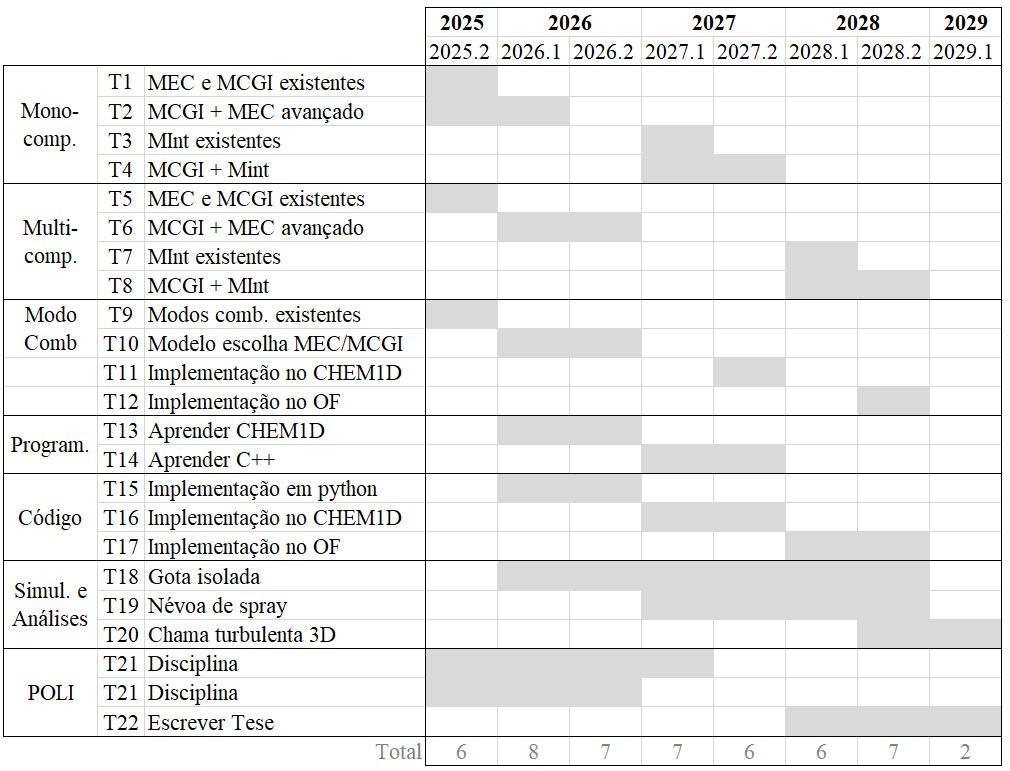
\includegraphics[width=0.99\textwidth]{30_images/cronograma-2.png}
    \label{fig:cronograma}
\end{figure}

% \subsection{Disciplinas a serem cursadas} \label{sec:disciplinas}


